\documentclass[11pt, a4paper]{article}

\usepackage{graphicx} 
\usepackage[utf8]{inputenc}
\usepackage{fancyhdr}
\usepackage{changepage}
\usepackage[onehalfspacing]{setspace}
\usepackage{ragged2e}
\usepackage{ amssymb, amsmath, amsthm, dsfont }
\usepackage[width = 18cm, top = 2.5cm, bottom = 3cm]{geometry}
\usepackage{extarrows}
% --------- Variabel, auf jedem Blatt ändern!
\newcommand{\blattnummer}{2}
\newcommand{\datum}{4. Mai 2017}
	% Punktezahlen & Summe
\newcommand{\p}{5}
\newcommand{\pp}{5}
\newcommand{\ppp}{10}
\newcommand{\pppp}{}
\newcommand{\sump}{20}
% --------- Macros

\newcommand{\myTitleString} {}
\newcommand{\myAuthorString} {}
\newcommand{\mySubTitleString} {}
\newcommand{\myDateString} {}

\newcommand{\myTitle}[1] {\renewcommand {\myTitleString}{#1}}
\newcommand{\mySubTitle}[1] {\renewcommand {\mySubTitleString}{#1}}
\newcommand{\myAuthor}[1] {\renewcommand{\myAuthorString}		{#1}}
\newcommand{\myDate}[1] {\renewcommand{\myDateString}{#1}}

\newcommand{\makeMyTitle}
{
\pagestyle{fancy}
\fancyhead[L]
{
\begin{tabular}{l}
\myTitleString
\\ \mySubTitleString 
\\ \myDateString
\end{tabular}
} 			
\fancyhead[C]{}
\fancyhead[R]{\myAuthorString}
\fancyfoot[C]{\thepage}
}

\setlength{\headheight}{45pt}

\makeatletter
\renewcommand*\env@matrix[1][*\c@MaxMatrixCols c]{%
  \hskip -\arraycolsep
  \let\@ifnextchar\new@ifnextchar
  \array{#1}}
\makeatother

    % args: Aufgabennummer, erreichbare Punkte
\newcommand{\aufgabe}[2] {\section*{Aufgabe \blattnummer.#1 (Punkte:\qquad/#2)}}
\newcommand{\aufgabenteil}[1] {\textbf{(#1)}}
% ---------
%\setlength{\parindent}{0pt}
\begin{document}

\myTitle{\textsc{Datenbanken und Informationssysteme}}
\mySubTitle{Übung \blattnummer}
\myDate{\datum}
\myAuthor
{
\begin{tabular}{l l}
359109, &Michelle Milde\\
356148, &Philipp Hochmann\\
356092, &Daniel Schleiz
\end{tabular}
}
\makeMyTitle

\hfill
\begin{tabular}{|c|c|c|c|}\hline
   1 & 2 & 3 & $\sum$\\\hline
  	 \qquad/\p & \qquad/\pp & \qquad/\ppp & \qquad/\sump\\\hline % abhängig vom Übungsblatt
 \end{tabular}
\hfill Korrigiert am:\underline{\hspace{3cm}}
\hfill
\vspace*{30pt}


\aufgabe{1}{\p}
\begin{figure}[H]
  \centering
  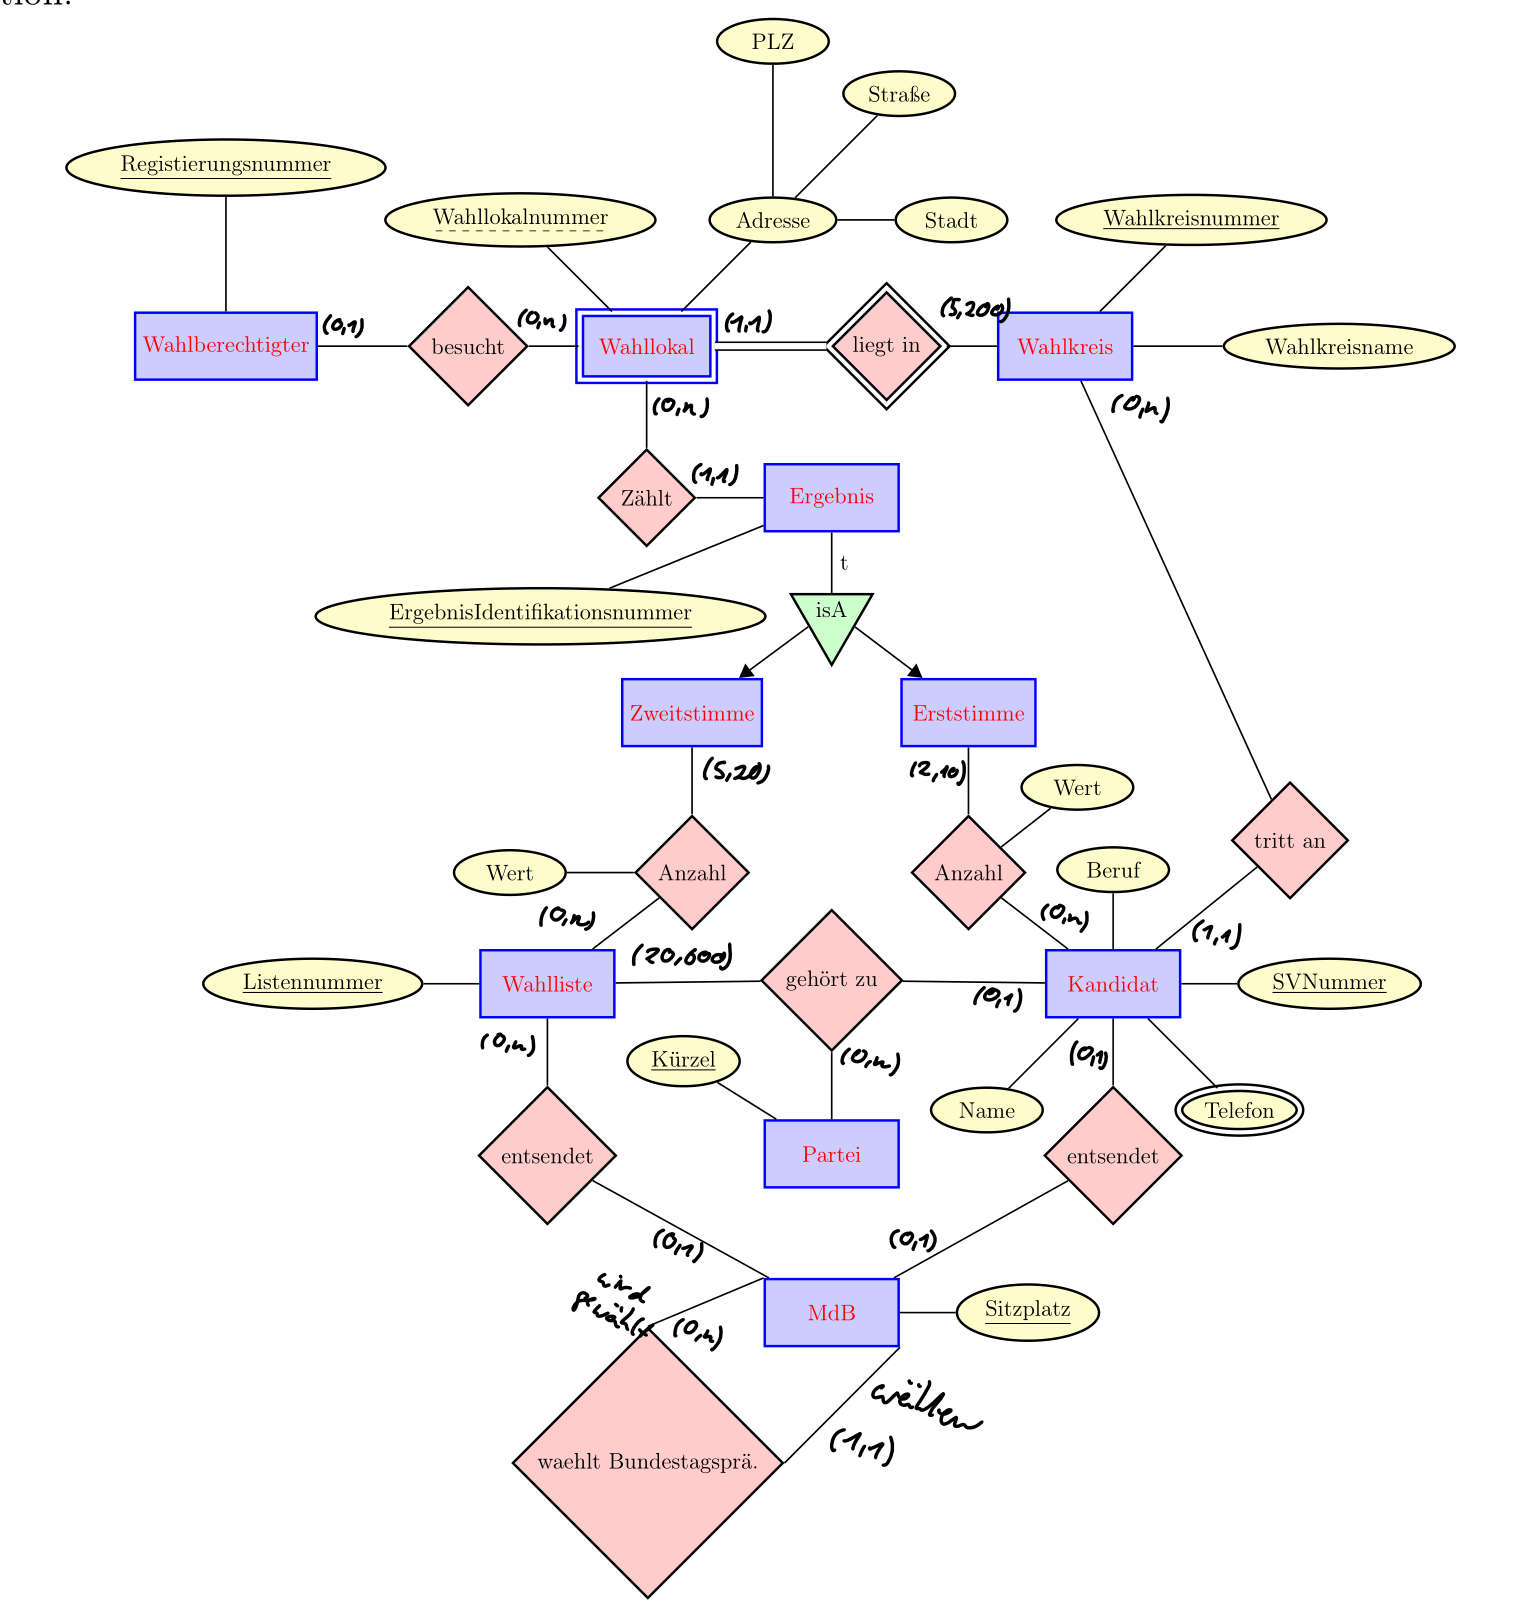
\includegraphics[width=\textwidth]{a1.png}
\end{figure}\
\newpage



\aufgabe{2}{\pp}
\begin{figure}[H]
  \centering
%  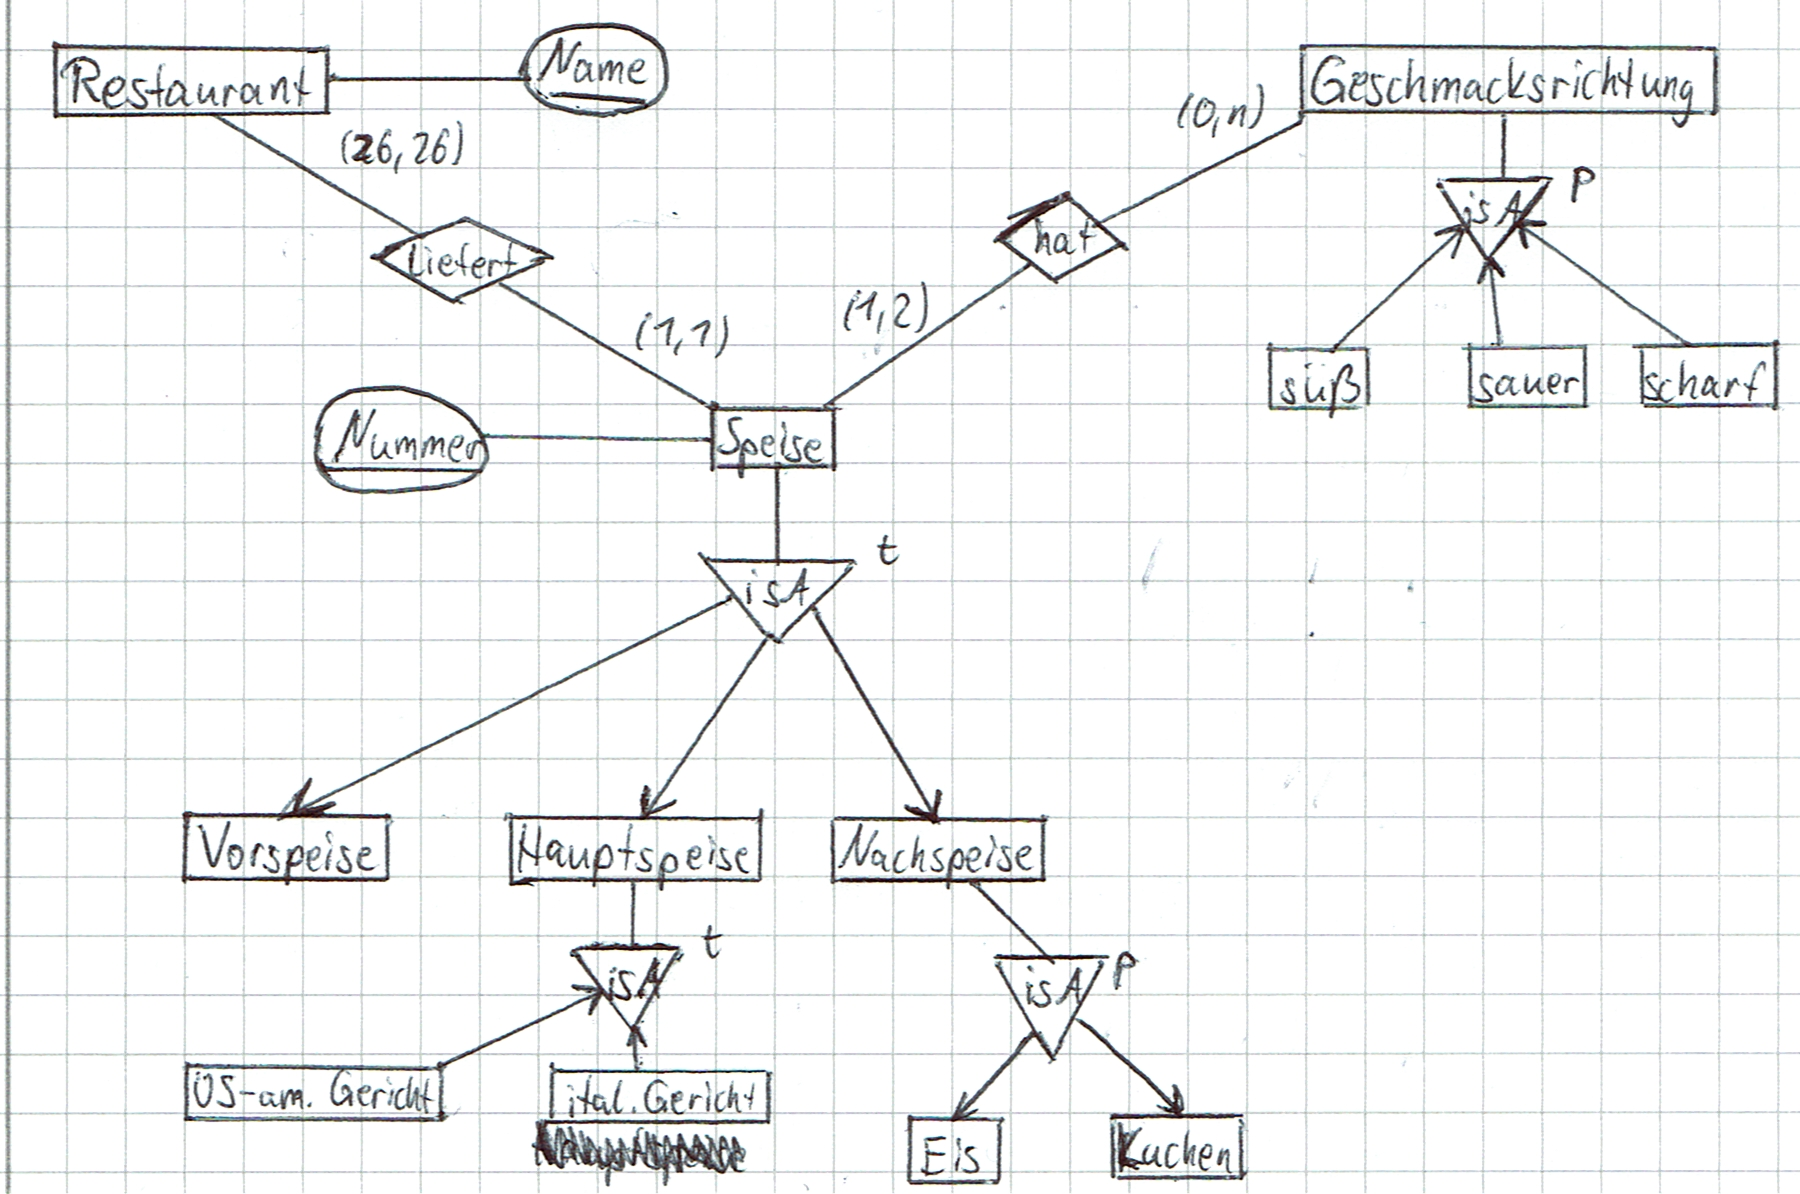
\includegraphics{a2.png}
\end{figure}\





\aufgabe{3}{\ppp}
\textbf{Relationenschema R}
\begin{adjustwidth}{20pt}{20pt}
Sportverband(\underline{Kürzel}, Nation)\\
Trainer(\underline{TID}, Name, Berufserfahrung)\\
Lizenz(\underline{Bezeichnung})\\
Verein(\underline{VID}, Name, Stadt)\\
Mannschaft(\underline{Kennzeichnung}, VID, TID)\\
Positionen(\underline{PID})\\
Feldspieler(\underline{SID}, Name, Alter, Mannschaftskennzeichnung, PID)\\
Torhüter(\underline{SID}, Name, Alter, Mannschaftskennzeichnung, Gegentore)\\
SpieltGegen(\underline{Ergebnis}, \underline{Datum})\\
AusgebildetVon(\underline{TID}, \underline{Bezeichnung}, Verbandskürzel)\\
\end{adjustwidth}

\textbf{Interrelationale Abhängigkeiten}
\begin{adjustwidth}{20pt}{20pt}
Feldspieler[Mannschaftskennzeichnung] $\subseteq$ Mannschaft[Kennzeichnung]\\
Torhüter[Mannschaftskennzeichnung] $\subseteq$ Mannschaft[Kennzeichnung]\\
\ \\
Feldspieler[SID] $\subseteq$ Spieler[SID]\\
Torhüter[SID] $\subseteq$ Spieler[SID]\\
\ \\
SpieltIn[SID] $\subseteq$ Feldspieler[SID] $\cup$ Torhüter[SID]\\
Feldspieler[SID] $\cap$ Torhüter[SID] $= \o$
SpieltGegen[Datum] $\subseteq$ Mannschaft[Kennzeichnung]\\
SpieltGegen[Ergebnis] $\subseteq$ Mannschaft[Kennzeichnung]\\
\ \\
Mannschaft[VID] $\subseteq$ Verein[VID]\\
\ \\
Mannschaft[TID] $\subseteq$ Trainer[TID]\\
\ \\
BildetAus[TID] $\subseteq$ Trainer[TID]\\
BildetAus[Kürzel] $\subseteq$ Sportverband[Kürzel]\\
BildetAus[Bezeichnung] $\subseteq$ Lizenz[Bezeichnung]\\
\end{adjustwidth}
% --------
\end{document}
